\newpage

\textbf{Validación del Eje.}

Para validar las dimensiones calculadas se procedió a hacer una simulación de estudio estático en SolidWorks.

Para ello se toma en consideración los puntos fijos, que representan lo rodamientos de apoyo, así como la fuerza ejercida por La banda de transmisión, además del par torsor al que esta sometido a lo largo del eje.

Para un estudio de esfuerzos aplicando el criterio de Von Mises (Figura \ref{fg:Esfuerzos}). 

\begin{figure}[h]
    \centering
        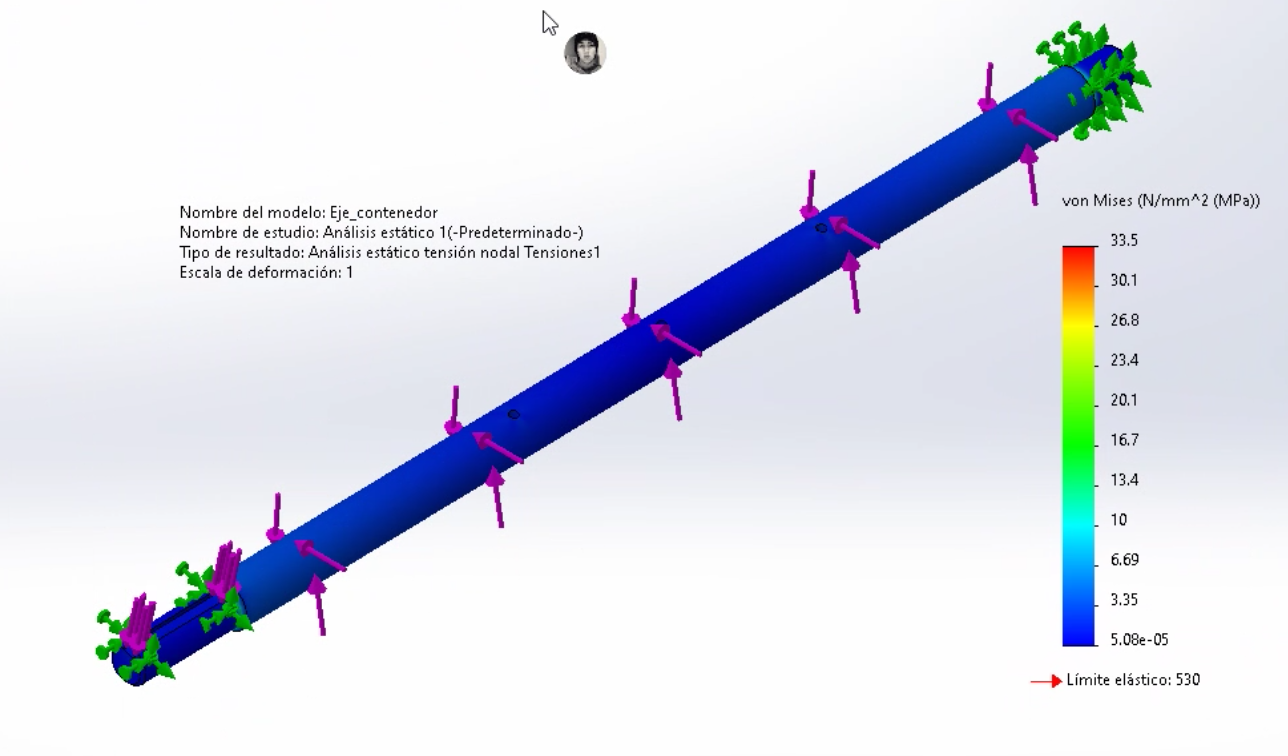
\includegraphics[scale=0.5]{images/Capitulo 4/s5/S5 validacion/Estudio Esfuerzos.png}
        \caption{Estudio Esfuerzos}
    \label{fg:Esfuerzos}
\end{figure}

Porque de la gráfica se observar que no existen puntos críticos en el eje, por lo que el eje no sufre riesgos de ruptura.